\documentclass[a4paper]{article}

\usepackage[english]{babel}
\usepackage[utf8x]{inputenc}
\usepackage{amsmath}
\usepackage{graphicx}
\usepackage[colorinlistoftodos]{todonotes}
\usepackage{array}

\title{Milestone 1: Project abstract}
\author{
  Berenji, Sarah\\
  \texttt{sarah.berenji@gmail.com}
  \and
  Forstén, Andreas\\
  \texttt{andreasforsten@gmail.com}
  \and
  Leskelä, Hannes\\
  \texttt{hleskela@kth.se}
  \and
  Letzner, Josefine\\
    \texttt{joletzner@gmail.com}
}
\date{2015-09-18}
\begin{document}
\maketitle
\section*{{Project description}}

We've chosen to do a version of the text analyser project, where we focus on categorizing either the content of the text or the type of text, depending on the difficulty level of the two alternatives. We will do this by implementing a heuristic that uses hidden Markov models, where we will research which variables should be included and give them a certain weight. If we have enough time, we will try to improve the heuristic by applying some sort of machine learning to the heuristic. If this is the case, it will probably be a simple version of policy gradient reinforcement learning (pgrl). We will work in python \textgreater= 3.0 and use some sort of natural language library to do the statistical analysis of the texts. Example libraries are TextBlob (https://textblob.readthedocs.org/en/dev) and the Natural Language Tool Kit (http://www.nltk.org)
\newline

\noindent The project plan can be seen in figure 1 below. The different activities contain the following:\\
Milestone 2, do research - During this time every group member will read about the subject in general, find references from previous work done related to our project and read/learn about the basics of the blob library and other useful tools that may show up during this work.\\
Milestone 2, write report - This time will be spent on writing a report draft based upon the previous research. The partitioning of work load between group members for this part is still to be planned.\\
Milestone 3, write code - This part is when we plan, again based upon the conclusions of our research, what the first draft of our code will look like and implement this. Depending on what difficulties that arise (which determines time left) a different number of techniques or refining of the existing techniques will be done. \\
Milestone 3, finish report - Soon after the coding has begun the report writing will continue and run in parallel. Results and conclusions will be written into the report as they emerge.\\
The other enteries seen in the gannt chart are preparation of presentation and meetings. The meetings will in the first place be held to plan in detail what every group member will work on until next meeting is held, to check upon what has happened since last time and to discuss the method. The workload is supposed to be spread even during over the project period.
  

\begin{figure}[t]

\hspace*{-1.5in}
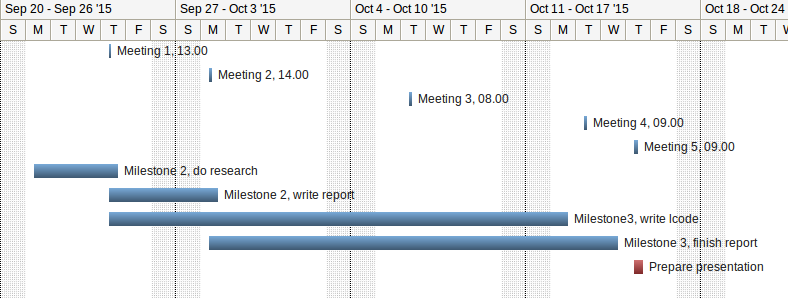
\includegraphics[scale=0.7]{gannt.png}
\textbf{Figure 1}
\end{figure}




\newpage
\section*{Updated project plan}
\begin{center}
    \begin{tabular}{| m{2cm} | m{8cm} | p{2cm} | p{2cm} |}
    \hline
    Person(s) & Task & Time(per person) & Deadline\\ \hline
    Ha + Sa & Create Parser & 8 h & oct 5\\ \hline
    Jo + An & Fetch data with Block Spring & 8 h & oct 5 \\ \hline
    Jo + An  & Investigate trainer (find out what the best training is in TextBlob) then train the analyser and write this to report & 14h & oct 5\\ \hline
    Ha + Sa & Investigate tester then test  & 5 h & oct 5\\ \hline
    Ha + Sa & Investigate word statistics (what should it extract) and implement reinforcement learning & 15 h & oct 12 (in case of time)\\ \hline
    Jo + An & Compare analyser v.s training + testing & 14 & oct 14\\ \hline
    Ha + Sa & Generate relevant graphs and statistics & 6 h & oct 14\\ \hline
    Jo + An & Write report: Complete background & 3 h & oct 5\\ \hline
    Ha + Sa & Write report: method (5 hours while working with the code and the rest later) & 5h + 5h &  10 oct\\ \hline
    Everyone & Write report: Discussion & 7 h & 15 oct\\ \hline
    Everyone & Prepare presentation & 7 h & 17 oct\\ \hline
    Everyone & Meetings & 5 x 3 h & 
    \end{tabular}
\end{center}

\end{document}
